This section describes the entire model formally using the alloy language.
In particular, we aim to model the relationships between entities that are used in the management of internships, such as students, companies and universities. Furthermore, we aim to ensure consistency by introducing the constraints that enable the creation and management of all processes in the system


\section{Alloy Code}
\lstinputlisting[language=alloy]{alloy/model.als}
\pagebreak

\section{Models}
\begin{enumerate}[label=,leftmargin=0cm]
      \item \textbf{Student participates in an internship}

            This model was generated using:
            \begin{lstlisting}[language=alloy]
            run {
                #Student = 2
	        #Company = 1
	        #Internship = 1
	        some i: Internship | i.state = InProgress
	        #Preferences >= 4
            } for 10
	
          \end{lstlisting}

            \begin{adjustbox}{max size={\textwidth}{\textheight}}
                  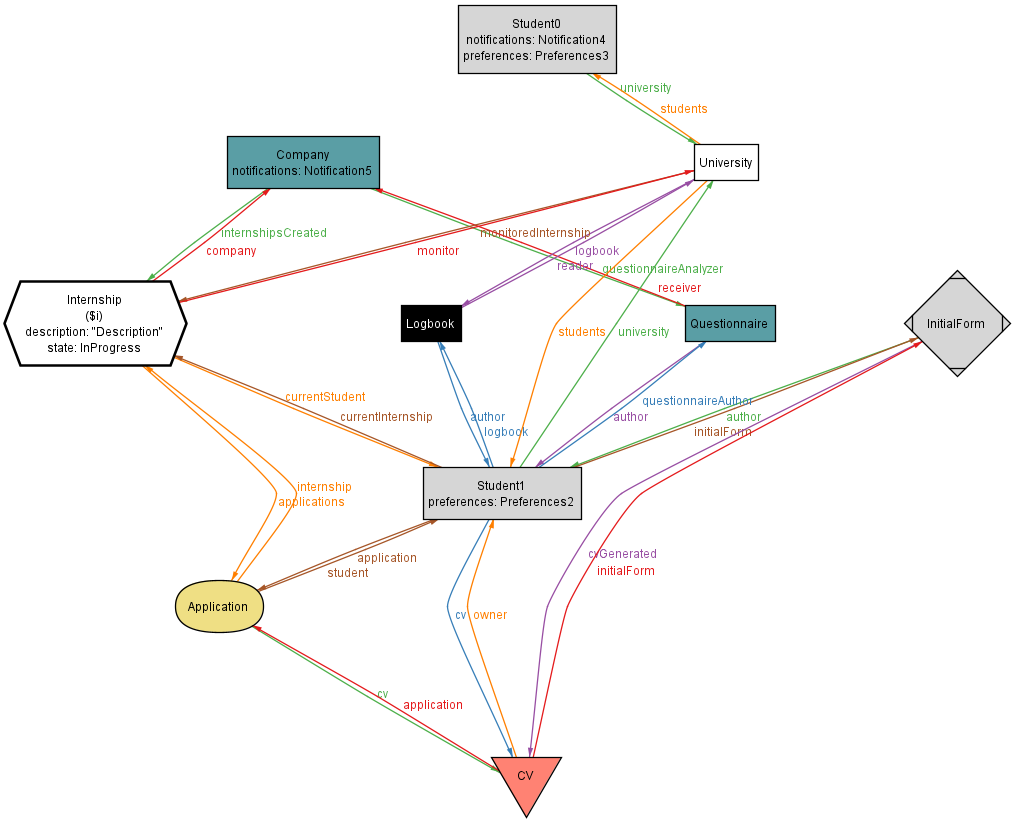
\includegraphics{alloy/alloy1.png}
            \end{adjustbox}

            This diagram shows us 2 students belonging to the same university. One of the two students is doing an internship at a company, and it shows us that this student had to fill out an ‘Initial Form’ in order to produce the CV that was used to make the application. The student also had to fill in a questionnaire at the selection stage and now has a logbook where he notes what he does in the company.

        \pagebreak
        \item \textbf{Company makes a report}

            This model was generated using:
            \begin{lstlisting}[language=alloy]
            run {
	        #Student = 3
	        #Company = 3
                #Internship = 3
                some i: Internship | i.state = InProgress
                #Preferences >= 4
                #ChatMessage >= 1
                #Report = 1
            } for 10
	
          \end{lstlisting}

            \begin{adjustbox}{max size={\textwidth}{\textheight}}
                  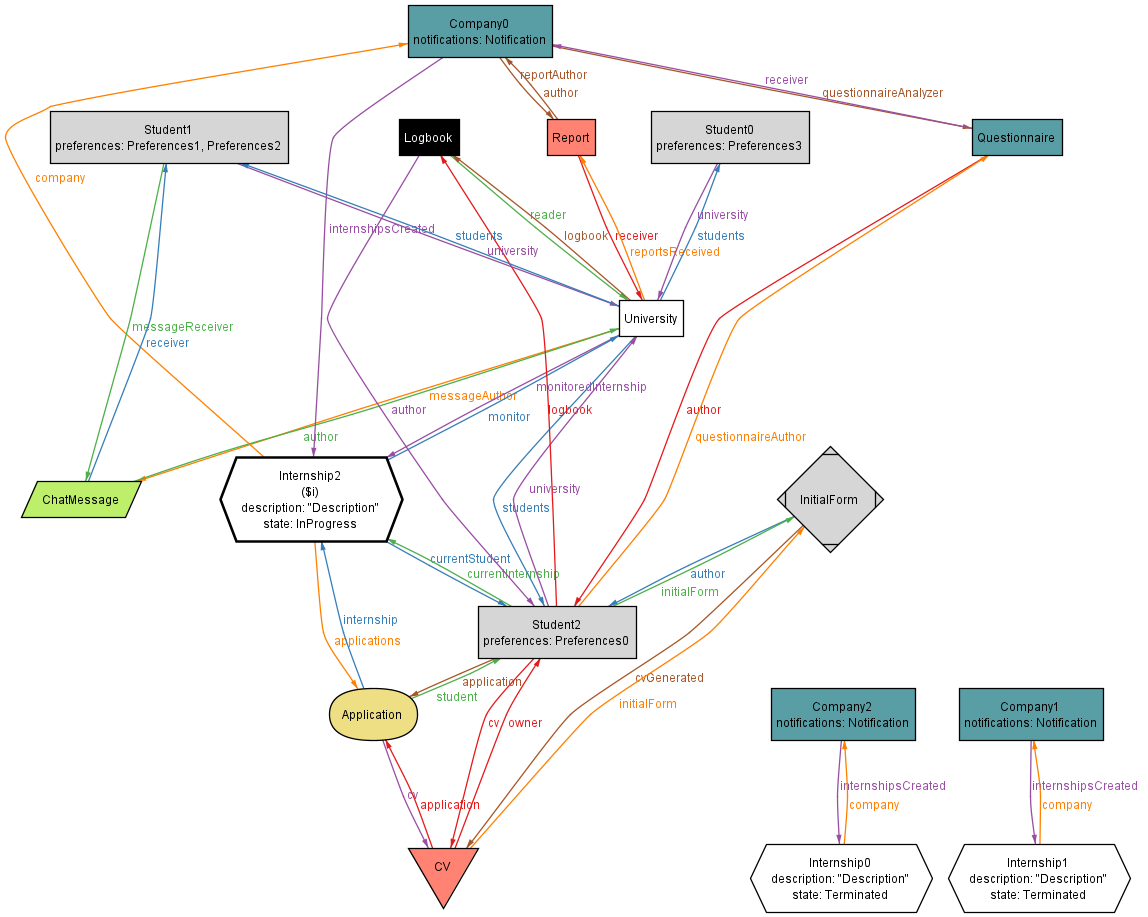
\includegraphics{RASD/alloy/alloy2.png}
            \end{adjustbox}

            This diagram shows us Student2 doing the Internship2, and he has in fact filled in an InitialForm and made the application (thus generating a CV). We also see that Company0, responsible for Internship2 has made a report to the university, probably reporting insufficient work by the student. We also see that Student1 has communicated with his university via chat. Finally, we can see that 2 other companies have created 2 internships which are now both terminated and therefore no longer have students
\end{enumerate}